        \documentclass{standalone}
        \usepackage{tikz}
        \begin{document}
        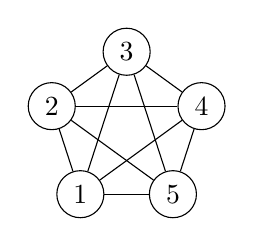
\begin{tikzpicture}


\centering
\tikzstyle{vertex}=[circle,draw,minimum size=17pt,inner sep=0pt]
  \foreach \name/\angle/\text in {P-1/234/1, P-2/162/2, P-3/90/3, P-4/18/4, P-5/-54/5}
    \node[vertex,yshift=.5cm] (\name) at (\angle:1cm) {$\text$};
  \foreach \from/\to in {1/2,2/3,3/4,4/5,5/1,1/3,2/4,3/5,4/1,5/2}
    { \draw (P-\from) -- (P-\to); }

        \end{tikzpicture}
        \end{document}
